%!TEX TS-program = xelatex
%!TEX program = xelatex
%!TEX encoding = utf8
%!TEX spellcheck = en_US
%!BIB program = bibtex




\documentclass[12pt,oneside,letterpaper]{article}

\nonstopmode

% Set a better default text area (note: don't use this and geometry at the same time.)
% \usepackage[DIV=10]{typearea}
\usepackage[margin=1.5in]{geometry}
\usepackage{fontspec}
\defaultfontfeatures{Ligatures=TeX}
\usepackage{amsmath}  % must be loaded before unicode-math
\usepackage{amsthm}
% Libertinus code suggested by https://tex.stackexchange.com/a/364502
\usepackage[
    math-style=ISO,
    bold-style=ISO,
    partial=upright,
    nabla=upright
]{unicode-math}
\setmainfont[Numbers={OldStyle, Proportional}]{Libertinus Serif}
\setsansfont{Libertinus Sans}
\setmathfont{Libertinus Math}
\newfontface\titlefont{Libertinus Serif Display}[Numbers={OldStyle, Proportional}, Fractions=Off,Ligatures=Common]
\newfontface\textfracfont{Libertinus Serif}[Numbers={OldStyle, Proportional}, Fractions=On]
\newfontface\tabularoldstylefont{Libertinus Serif}[Numbers={OldStyle, Monospaced}, Fractions=Off]

\usepackage{csquotes}
\usepackage[final]{microtype}
\frenchspacing{}
\microtypecontext{spacing=french}

\usepackage{ragged2e}  % allow for ragged-right with hyphenation

% Format sections:
% \titleformat{command}[shape]{format}{label}{sep}{before-code}[after-code]
\usepackage[it, small]{titlesec}

% Format itemized lists
\usepackage{enumitem}
\setlist{nolistsep} % more aggressive than noitemsep

% allow page breaks in math equations
\allowdisplaybreaks

\newcounter{axiomcounter}
\newcounter{theoremcounter}
\newcounter{examplecounter}
\newcounter{propositioncounter}
\newcounter{lemmacounter}
\newcounter{corollarycounter}

% Make it easier to change the spacing around these math environments
\newlength{\premathenv}
\setlength{\premathenv}{0.2\baselineskip}
\newlength{\withinmathenv}
\setlength{\withinmathenv}{0\baselineskip}
\newlength{\postmathenv}
\setlength{\postmathenv}{\premathenv} % default to the same, but could change.


\newcommand{\norm}[1]{\left\lVert#1\right\rVert}
\newcommand{\length}[1]{\left\lvert#1\right\rvert}

\theoremstyle{definition}
\newenvironment{theorem}[1]{%
\vspace{\premathenv}%
\refstepcounter{theoremcounter}%
\noindent\textbf{Theorem \thetheoremcounter}
{#1}
\vspace{\withinmathenv}
}{% end of beginning of environment, beginning of end of env
\vspace{\postmathenv}%
}
\newenvironment{proposition}[1]{%
\vspace{\premathenv}%
\refstepcounter{propositioncounter}%
\noindent\textbf{Proposition \thepropositioncounter}
{#1}
\vspace{\withinmathenv}
}{% end of beginning of environment, beginning of end of env
\vspace{\postmathenv}%%
}
\newenvironment{lemma}[1]{%
\vspace{\premathenv}%
\refstepcounter{lemmacounter}%
\noindent\textbf{Lemma \thelemmacounter}
{#1}
\vspace{\withinmathenv}
}{% end of beginning of environment, beginning of end of env
\vspace{\postmathenv}%
}
\newenvironment{corollary}[1]{%
\vspace{\premathenv}%
\refstepcounter{corollarycounter}%
\noindent\textbf{Corollary \thecorollarycounter}
{#1}
\vspace{\withinmathenv}
}{% end of beginning of environment, beginning of end of env
\vspace{\postmathenv}%
}
\newenvironment{axiom}[1]{%
\vspace{\premathenv}%
\refstepcounter{axiomcounter}%
\noindent\textbf{Axiom \theaxiomcounter}
{#1}
\vspace{\withinmathenv}
}{% end of beginning of environment, beginning of end of env
\vspace{\postmathenv}%
}
\newenvironment{example}[1]{%
\vspace{\premathenv}%
\refstepcounter{examplecounter}%
\noindent\textbf{EXAMPLE \theexamplecounter}
{#1}
\vspace{\withinmathenv}
}{% end of beginning of environment, beginning of end of env
\vspace{\postmathenv}%
}

\renewenvironment{proof}{%
\vspace{\premathenv}% previously \vspace{1\baselineskip}
\noindent{\textit{Proof:} }
}{% end of beginning of environment, beginning of end of env
\qed
\vspace{\postmathenv}% previously \vspace{1\baselineskip}
}
\newtheorem{case}{Case}
\renewcommand*{\thecase}{\Alph{case}}
\newtheorem{assumption}{Assumption}
\renewcommand*{\theassumption}{\Alph{assumption}}

\def\equationautorefname~#1\null{(#1)\null}

\newcounter{auditpolicy}
\setcounter{auditpolicy}{-1}
\newenvironment{auditpolicy}[1]{%
\refstepcounter{auditpolicy}%
{\tabularoldstylefont(\theauditpolicy)}~#1%
}


\usepackage{fancyhdr}
\pagestyle{fancy}
\lhead{}
\chead{}
\rhead{}
\lfoot{}
\cfoot{}
\rfoot{\thepage}
\renewcommand{\headrulewidth}{0pt}
\usepackage{xcolor}

% Redefine \left and \right with better spacing
\usepackage{mleftright}
\mleftright{}

% Define \expected and \indicator commands
\DeclareMathOperator{\blackboardE}{\mathbb{E}}
\newcommand{\expected}[1]{\blackboardE\left[#1\right]}
\newcommand{\indicator}[1]{\symbf{1}\left[#1\right]}



\usepackage{rotating} % provide the sidewaysfigure environment

% Set up tables
\usepackage[online,flushleft]{threeparttable}
\usepackage{dcolumn}
\newcolumntype{d}{D{@}{\hspace{0pt}}{4}}
\newcommand{\textcol}[1]{\multicolumn{1}{c}{#1}}

% \usepackage{sparklines}
\usepackage{tabularx}
\usepackage{longtable}
\usepackage{booktabs}

% Bibliography
\usepackage[
  authordate,
  isbn=false,
  backend=bibtex,
  autopunct=true,
  uniquename=false
  % backref=true
]{biblatex-chicago}
\renewcommand*{\bibfont}{\small}
\addbibresource{refs.bib}
\addbibresource{data_cites.bib}
\addbibresource{methane_measurement_refs.bib}

% use the \ce{} command for chemistry expressions like \ce{CO2}
\usepackage[version=4]{mhchem}

\usepackage{nameref}

% Set up a boolean so we can easily turn endfloat on and off.
% To turn on, change to \togglefalse{endfloat}
\newtoggle{endfloat}
\togglefalse{endfloat}
\iftoggle{endfloat}{%
  \usepackage{endfloat}
  % stopendfloat from putting everything on separate pages
  \renewcommand{\efloatseparator}{\mbox{}}
}{ % else :
  \usepackage{placeins} % provide \FloatBarrier command
}

% Define a boolean for whether we'll use the xr package.
\newtoggle{usexr}

\usepackage{graphicx}
\graphicspath{{../graphics/}}
\usepackage{import} % better relative import paths
\usepackage{tikz}
\usetikzlibrary{calc}
\usepackage{wrapfig} % provides wrapfigure and wraptable environments


% Define a command \blfootnote (blind foodnote or blank footnote)
% Redefine \thefootnote to remove the symbol
% Redefine \@makefntext to try to mimic the biblatex-chicago option footmarkoff, but only for the scope of this command.
% Then reset the counter.
\makeatletter
\newcommand{\blfootnote}[1]{%
  \begingroup
  \renewcommand{\thefootnote}{}%
  \renewcommand{\@makefntext}{}%
  \footnote{#1}%
  \addtocounter{footnote}{-1}%
  \endgroup
}
\makeatother


% Add an orcid logo:
% Borrowed partly from https://tex.stackexchange.com/a/445583
% And downloaded graphic from
% https://figshare.com/articles/ORCID_iD_icon_graphics/5008697
\usepackage{scalerel}
\newcommand\orcidicon[1]{\href{https://orcid.org/#1}{\mbox{\scalerel*{

\includegraphics{ORCIDiD_iconvector.pdf}
}{|}}}}


% Run texcount shell command and input result. Requires shell escape (or restricted shell escape) and associated security warnings
% The -merge option includes counts for any \input{}-ed files.
%\usepackage{shellesc}
%\newcommand{\wordcount}[1]{%
%\input|"texcount -1 -sum -merge -q #1.tex"%
%}


\usepackage{setspace}
\onehalfspacing
\usepackage{footmisc} % must be loaded before hyperref; allows references to footnotes.

\usepackage{url} % better URL line breaks.
% Ensure more achievable output (font embedding etc.) but see the docs about
% what it takes to be PDF/A-3b compliant.
% \usepackage[a-3b]{pdfx}



% Make hyperref happy. https://tex.stackexchange.com/a/256677
\providecommand*\propositioncounterautorefname{proposition}

\widowpenalty 9999
\predisplaypenalty=0 % lower than default 10000


%----Helper code for dealing with external references----
% (by cyberSingularity at http://tex.stackexchange.com/a/69832/226)
% https://www.overleaf.com/learn/how-to/Cross_referencing_with_the_xr_package_in_Overleaf

\makeatletter

\newcommand*{\addFileDependency}[1]{% argument=file name and extension
\typeout{(#1)}% latexmk will find this if $recorder=0
% however, in that case, it will ignore #1 if it is a .aux or
% .pdf file etc and it exists! If it doesn't exist, it will appear
% in the list of dependents regardless)
%
% Write the following if you want it to appear in \listfiles
% --- although not really necessary and latexmk doesn't use this
%
\@addtofilelist{#1}
%
% latexmk will find this message if #1 doesn't exist (yet)
\IfFileExists{#1}{}{\typeout{No file #1.}}
}\makeatother

\newcommand*{\myexternaldocument}[1]{%
\externaldocument{#1}%
\addFileDependency{#1.tex}%
\addFileDependency{#1.aux}%
}
%------------End of helper code--------------



% Note that JAERE does not support this - so the toggle is off in the paper
\toggletrue{usexr}
\iftoggle{usexr}{%.
  \usepackage{xr}
  \myexternaldocument{paper}
}{}

\renewcommand{\thesection}{A\arabic{section}}
\renewcommand{\thetable}{A\arabic{table}}
\renewcommand{\thefigure}{A\arabic{figure}}

% In addition to shared cites files in the paper_appendix_shared_preamble
\addbibresource{software_cites_r.bib}
\addbibresource{software_cites_python.bib}

% Load hyperref last
\usepackage{hyperref}
\hypersetup{colorlinks,
  linkcolor=blue!40!black,
  filecolor=black,
  urlcolor=blue!40!black,  % 40% blue, 60% black
  citecolor=black,
  pdfpagemode=UseNone,
  pdftoolbar=false,
  pdftitle={},
  pdfauthor={},
  pdfsubject={},
  pdfcreator={},
  pdfproducer={},
  pdflang=en,
  unicode=true
}



% Write out acronyms in small caps that can be copy-pasted as full caps.
% It would be nice to have something that depended less on defining each acronym, or less on the c2sc OpenType font feature
% Usage: \makeacronym{NASA}
\usepackage{accsupp}
\usepackage{glossaries}
\glsdisablehyper{} % disable hyperlinks


% Create acronyms in a way that works nicely with smallcaps.
% (eg \setacronymstyle{long-sc-short})
% This code makes the acronym lowercase so small caps can be applied,
% but adds an accessibility layer so it copies-pastes in upper case.
\newcommand{\makeacronym}[2]{%
\newacronym{#1}{%
\protect\BeginAccSupp{method=plain,ActualText=#1}%
\MakeLowercase{#1}%
\protect\EndAccSupp{}%
}{#2}%
}
\makeacronym{ARE}{Agricultural and Resource Economics}
\makeacronym{AVIRIS-NG}{``next generation airborne visible/infrared imaging spectrometer''}
\makeacronym{BAU}{business as usual}
\makeacronym{BLS}{Bureau of Labor Statistics}
\makeacronym{CDD}{cooling degree days}
\makeacronym{CDF}{cumulative distribution function}
\makeacronym{CEMS}{continuous emissions monitoring}
\makeacronym{CI}{confidence interval}
\makeacronym{DBSCAN}{density-based spatial clustering of applications with noise}
\makeacronym{DWL}{deadweight loss}
\makeacronym{EPA}{Environmental Protection Agency}
\makeacronym{EU ETS}{European Union Emission Trading Scheme}
\makeacronym{FOC}{first-order condition}
\makeacronym{GDP}{gross domestic product}
% \makeacronym{FEAST}{}
% Could make GHG have a proper plural: https://tex.stackexchange.com/a/128419
\newacronym[longplural={greenhouse gases}, shortplural={ghg}]{GHG}{%
\protect\BeginAccSupp{method=plain,ActualText=GHG}%
ghg%
\protect\EndAccSupp{}
}{greenhouse gas}
\makeacronym{GHGI}{greenhouse gas inventory}
\makeacronym{GHGRP}{greenhouse gas reporting program}
\makeacronym{GOSAT}{Greenhouse Gases Observing Satellite}
\makeacronym{GWP}{global warming potential}
\makeacronym{HDD}{heating degree days}
\makeacronym{i.i.d.}{independent and identically distributed}
\makeacronym{IHS}{inverse hyperbolic sine}
\makeacronym{IPCC}{Intergovernmental Panel on Climate Change}
\makeacronym{KKT}{Karush–Kuhn–Tucker}
\makeacronym{LDAR}{leak detection and repair}
\makeacronym{MCMC}{Markov chain Monte Carlo}
\makeacronym{MLE}{maximum likelihood estimation}
\makeacronym{MSE}{mean squared error}
\makeacronym{OSHA}{Occupational Safety and Health Administration}
\makeacronym{PDF}{probability density function}
\makeacronym{SCC}{social cost of carbon}
\makeacronym{SDID}{synthetic difference in differences}
\makeacronym{SNL}{SNL Financial}
\makeacronym{WAIC}{widely applicable information criterion}
 % loads glossaries package, and should be loaded after hyperref
\setacronymstyle{long-sc-short}

\begin{document}
\begin{center}

\
{\Large\titlefont
Online Appendix for ``Information Matters: Feasible Policies for Reducing Methane Emissions''
\vspace{6pt}

}
\vspace{1.5\baselineskip}


{\large\titlefont
Karl Dunkle Werner%
\textsuperscript{ \orcidicon{0000-0003-0523-7309}}
and Wenfeng Qiu%

% \today{}
August 21, 2024

\vspace*{1\baselineskip}

}% end of \large\titlefont

\end{center}



\section{Proofs and Technical Details}
\label{app:proofs}

\subsection{Proof of Proposition~\ref{prop_properties_of_dwl}}
\label{app:proofs-well-operator}
\begin{proof}
Because \(C_i'\) is strictly increasing and convex, \(C_i'^{-1}(x) =: f(x)\) is strictly increasing and concave.
\begin{align*}
\frac{\partial \text{DWL}_i}{\partial t_i} &= - \frac{\partial {C_i'}^{-1}(e_i \cdot (p_i + t_i))}{\partial t_i} \cdot e_i (\delta - t_i) = - f' \cdot e_i^2 (\delta - t_i) < 0\\
\frac{\partial^2 \text{DWL}_i}{\partial t^2_i} &= - \frac{\partial f' \cdot e_i^2 (\delta - t_i)}{\partial t_i} = -e_i^2(\underbrace{f'' \cdot e_i(\delta - t_i)}_{<0} - f') > 0
\end{align*}
\end{proof}


\subsection{Proof of Proposition~\ref{prop_monotone_audit}}
\label{app:audit-policy-proofs-covariates}
\begin{proof}
The feasible set under the constraint is a compact subset of \(\mathbb{R}^N\) so a solution exists.
Because \(\text{\gls{DWL}}_i\) only depends on \(r_i\) and \(\text{\gls{DWL}}_i\) is strictly increasing,
convex in \(r_i\) and the constraints are linear inequalities,
we conclude a unique solution exists and can be characterized by the standard \gls{KKT} conditions.

Let \(r^*_i\)s be the solution of the problem.
Suppose there exists \(k,j\) such that \(e_k > e_j\) but \(r^*_k < r^*_j\).
Consider \(\hat{r_i}\)s such that \(\hat{r_i} = r^*_i\) for all \(i \neq k,j\) and  \(\hat{r_k} = r^*_j, \hat{r_j} = r^*_k\).
Clearly, \(r^*_i\) also satisfy all the constraints.
The difference in the total \gls{DWL} for \(\hat{r_i}\)s and \(r^*_i\)s is equal to
\begin{align*}
&\text{DWL}_k(\hat{r_k}) + \text{DWL}_j(\hat{r_j}) - (\text{DWL}_k(r^*_k) + \text{DWL}_j(r^*_j))\\
= &\text{DWL}_k(r^*_j) - \text{DWL}_k(r^*_k) + \text{DWL}_j(r^*_k) - \text{DWL}_j(r^*_j)\\
= &\int_{r^*_k}^{r^*_j} \frac{\partial \text{DWL}_k}{\partial r_k} \ d r + \int_{r^*_j}^{r^*_k} \frac{\partial \text{DWL}_j}{\partial r_j} \ d r\\
= & \int_{r^*_k}^{r^*_j} \frac{\partial \text{DWL}_k}{\partial r_k} - \frac{\partial \text{DWL}_j}{\partial r_j} \ d r
\end{align*}
Since \(\frac{\partial^2 \text{DWL}_i}{\partial r_i \partial e_i} < 0\) and \(e_k > e_j\), the integrand is negative and hence the whole integral is negative, which implies \gls{DWL} under \(\hat{r_i}\)s is small.
This a contradiction to \(r^*_i\)s being optimal.
\end{proof}

Note that for the estimation part, the inequality \(\frac{\partial^2 \text{DWL}_i}{\partial r_i \partial e_i} < 0\) follows directly from the specific choice function we chose and the expected fee \(t_i\) being an increasing function of \(r_i\),
\begin{align*}
  \frac{\partial^2 DWL_i}{\partial t_i \partial e_i} &=
    \left(1 + \frac{1}{\alpha}\right) e^{\frac{1}{\alpha}}_i
    \frac{(\delta - t_i)}{\alpha (p_i + t_i)}
    \left(\frac{(p_i + t_i)}{A}\right)^{\frac{1}{\alpha}} < 0
\end{align*}

\subsection{Proof of Proposition~\ref{prop_value_of_info}}
\begin{proof}
Suppose there is no leak observed for a well.
Then the well operator will not pay any fee even when the well pad is audited because the leak detection threshold is the same for remote measurement and the audit under Policy 3a.
It follows that the regulator should not audit this well pad to save the audit budget.

Let \(r^*_i\)s be the optimal audit probabilities for Policy 2 so \(\sum^{N}_{i=1} r^*_i \leq M\).
Because \(0 \leq q_i \leq 1\), \(\sum^{N}_{i=1} \Bigl( q_i \cdot 0 + (1 - q_i) r^*_i \Bigl) \leq M\).
That is, every set of feasible audit probabilities \(r^*_i\)s for Policy 2 is also feasible for Policy 3a.
Since Policy 2 has the same objective function as Policy 3a, it follows the regulator achieves a higher \gls{DWL} reduction.
\end{proof}


\newpage

\subsection{Extensive form game trees for policies \ref{policy-target-x} and \ref{policy-target-e}a}



\begin{figure}[!pbth]
\vspace*{-1\baselineskip}%
\import{individual_figures/}{figureA01_game_tree_target_x.tex} % fig:game-tree-target-x

\begin{minipage}{1\textwidth}

\begin{justify}
{\small
In this figure, the well operator chooses the probability of not having a leak, \(q_i\), with full knowledge of the probability they will be audited, \(r_i\).
Then nature determines whether a leak occurs.
The regulator does not know whether a leak has occurred---their information set is indicated in a dashed oval.
If the well pad is leaking and is audited, the well operator pays \(\tau e_i\).
In all other cases, they pay zero.
}
\end{justify}
\end{minipage}
\end{figure}



\begin{figure}[!pbth] % fig:game-tree-target-e-no-censor
\import{individual_figures/}{figureA02_game_tree_target_e_no_censor.tex}

\begin{minipage}{1\textwidth}

\begin{justify}
{\small
In this figure, the well operator chooses the probability of not having a leak, \(q_i\), with full knowledge of the probability they will be audited, \(r_i\).
Then nature determines whether a leak occurs.
The regulator knows when a leak has occurred, and will never audit a well pad that isn't leaking.
If the well pad is leaking and is audited, the well operator pays \(\tau e_i\).
In all other cases, they pay zero.
}
\end{justify}
\end{minipage}
\end{figure}

\clearpage


\subsection{Policy~\ref{policy-target-e}b: Target auditing on observed emissions: high threshold}
\label{app:audit-target-e-high-threshold}

Policy~\ref{policy-target-e}b is the case where the regulator may observe very large leaks, over some detection threshold, then must decide which wells to audit.
Only wells that are audited and leaking are assessed a fee.
This policy is a generalization of policy~\ref{policy-target-e}a, which was the same but without a significant detection threshold.

Figure~\ref{fig:game-tree-target-e-censor} has a game tree for the regulator's problem.
Each well operator knows whether they're on the left branch (large~\(e_i\)) or right branch (small~\(e_i\)), since \(e_i\) is not a choice variable.
The dashed oval indicates the regulator's information set---they cannot tell whether a well pad has a large \(e_i\) and isn't leaking, a small \(e_i\) and isn't leaking, or a small \(e_i\) and is leaking.

\begin{figure}[!hbt]
\import{individual_figures/}{figureA03_game_tree_target_e_censor.tex}


\begin{minipage}{0.95\textwidth}

\begin{justify}
{\small
In this figure, nature determines the well's potential leak size, \(e_i\).
It is not a choice variable.
The well operator knows \(e_i\); the regulator can only form expectations.
The well operator chooses their probability of not having a leak, \(q_i\).
If a leak happens at a large well, it is detected.
If a leak happens at a small well, it is not.
If a leaking well pad is audited, it pays \(\tau e_i\).
The dashed oval indicates the regulator's information set.
}
\end{justify}
\end{minipage}
\end{figure}



The regulator sets audit probabilities based on whether the leakage is detected, taking
the detection threshold into account.
As the game tree suggests, if a well pad is \textit{not} detected with leakage, there is no way to distinguish between whether it is actually not leaking or the leakage is small.
As a result, the regulator can only specify an audit probability \(r_i(X_i)\) for a well pad \(i\) with detected leakage and an audit probability \(s_i(X_i)\) for a well pad with \textit{no} detected leakage (the covariates \(X\) included in the brackets means the \(r,s\) can depend on these covariates).

A well operator's response to this policy will depend on their \(e_i\).
For small-\(e\) wells, their response is straightforward; because they know they will always be audited with probability \(s_i\), the \gls{DWL} will be \(\text{\gls{DWL}}_i(s_i)\).
But for large wells, the incentives are more complicated.
A large well pad \(i\) will have \(q_i\) probability of \textit{not} leaking.
But even when it is not leaking, it will be audited with probability \(s_i(X_i)\).
Since it is not leaking, the audit will not lead to any penalty
(the auditing effort is wasted here).
Large-\(e\) wells will not care about \(s_i\).
\(q_i\) and \(\text{\gls{DWL}}_i\) will be functions that depend only on \(r_i\).
The \textit{ex-ante} \gls{DWL} for a large-\(e\) well pad will be
\(\text{\gls{DWL}}_i(r_i)\).

The budget is similar to the case with no detection threshold.
As with the \gls{DWL}, it's the probability of being audited \emph{when leaking} that matters to the well operator, so the large-\(e\) wells choose \(q_i(r_i)\) (\(s_i\) does not enter).
Unlike the previous cases, large-\(e\) wells now have some \(s_i\) probability of being audited when not leaking.
Therefore, the audit costs are \((1 - q_i(r_i)) r_i + q_i(r_i) s_i\) for each large-\(e\) well, and \(s_i\) for each small-\(e\) well.

Given these \gls{DWL} and budget components, the regulator needs to pick \(r_i\) and \(s_i\).
The regulator still does not know which wells are large-\(e\) or small-\(e\), so optimizes a weighted average, where the weights are the probability the well's leak is above the threshold.
For a detection threshold \(\underline{e}\), define
\(z_i \equiv \Pr(e > \underline{e} \mid X_i)\).
The regulator then optimizes the problem:
\begin{align*}
\min_{
\{r_i\}_{i = 1} ^ N, \{s_i\}_{i = 1} ^ N
} \quad &
\sum_i
z_i  \text{DWL}_i(r_i) +
(1 - z_i ) \text{DWL}_i(s_i)\\
&\textit{s.t. }
\sum_i
z_i [(1 - q_i(r_i)) r_i + q_i(r_i) s_i] +
(1 - z_i) s_i
\leq M\\
&\forall i: r_i \in [0, 1], s_i \in [0, 1]
\end{align*}
We can compare this minimization problem with the previous one, where \(\underline{e} = 0\), to confirm that the previous problem was a special case of this one.
In the previous problem, \(z_i\) converges to 1, so we do not need to worry about \(s_i\) in the objective function.
Moreover, in the budget constraint, \(s_i\) should be set to zero to save audit effort.
Lowering the detection threshold leads to a lower \gls{DWL}.


\newpage
\section{Methane Measurement}
\label{app:methane-measurement}

\begin{figure}[!hbtp]
\caption{Production segment is responsible for 58\% of leaks from natural gas supply chain}
\vspace*{1\baselineskip}

\label{fig:EPA-leak-percentages-Marks}

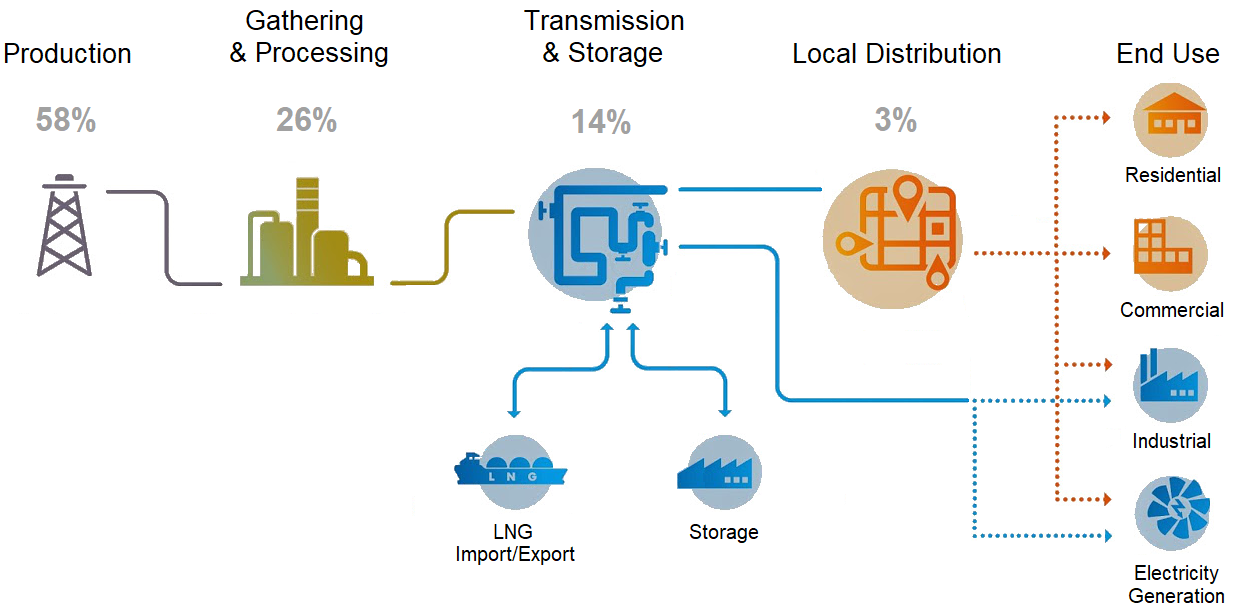
\includegraphics[width=\textwidth]{figureA04_natural_gas_leakage_percentages_marks_fig1}

\textsc{Source:} \textcite{Marks:2021} figure~1, from estimates in \textcite{Alvarez/etal:2018}.
Excludes end-use leaks.
\end{figure}

\begin{table}[!bth]
\centering
\import{individual_figures/}{tableA01_Cusworth_etal_2019_table2.tex}
\end{table}



\begin{figure}[!bth]
\caption{Distribution of detected methane leaks, comparison with ground-based measurement}
\label{fig:app-leak-sizes}
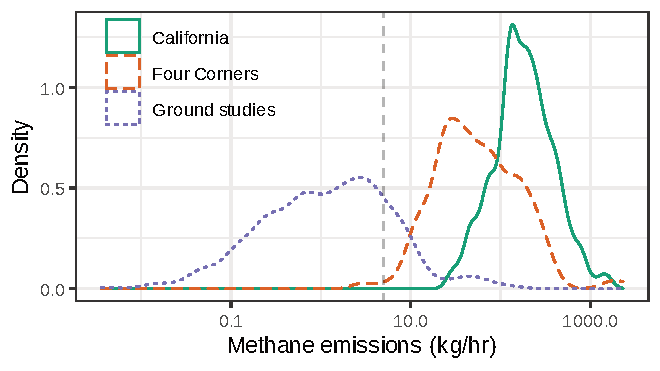
\includegraphics[width=0.49\textwidth]{figureA05_leak_comparison_sizes}
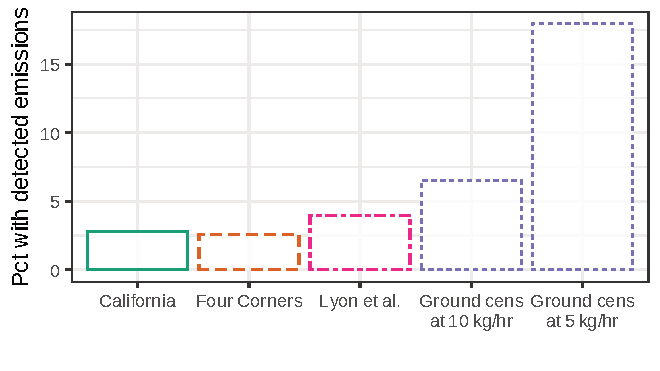
\includegraphics[width=0.49\textwidth]{figureA05_leak_comparison_fraction_with_detect}

\textsc{Left:} emissions conditional on detection.
\textsc{Right:} fraction of well pads with detected emissions.
The ``ground cens at'' columns are the ground studies' observations with artificial censoring applied, at either 5~or 10~kg/hr, the approximate detection threshold of both the California and Four Corners studies.
Without artificial censoring, the ground-based measurements are non-zero approximately 97\% of the time.
% Unrounded: 96.73913%
5~kg/hr is noted with a dashed line in the left plot.

\textsc{Sources:}
Ground studies include measurements primarily from
\textcite{Robertson/Edie/Snare/Soltis/Field/Burkhart/Bell/Zimmerle/Murphy:2017}
with additional contributions from
\textcite{
Rella/Tsai/Botkin/Crosson/Steele:2015,
Omara/Sullivan/Li/Subramanian/Robinson/Presto:2016,
Omara/Zimmerman/Sullivan/Li/Ellis/Cesa/Subramanian/Presto/Robinson:2018,
}.

California and Four Corners distributions come from aircraft studies \parencite{Duren/etal:2019, Frankenberg/etal:2016}.
\textcite{Lyon/Alvarez/Zavala-Araiza/Brandt/Jackson/Hamburg:2016}
provides information about leak prevalence (with a detection threshold roughly similar to the California and Four Corners studies), but not leak size.
\end{figure}



\begin{table}[!bth] % \ref{tab:covariate-balance-comparison}
\import{individual_figures/}{tableA02_covariate_balance_comparison_detect_leak.tex}
\end{table}


\begin{figure}[!hbt] % \ref{fig:frankenberg-measurement-figs}
\import{individual_figures/}{figureA06_frankenberg_measurement_figs.tex}
\end{figure}


\begin{figure}[!hbt] % \ref{fig:nat-gas-price-timeseries}
\import{individual_figures/}{figureA07_nat_gas_price_timeseries.tex}
\end{figure}


\begin{figure}[!hbt] % \ref{fig:nat-gas-price-timeseries}
\caption{Matched natural gas prices exhibit little variation}
\label{fig:nat-gas-price-histogram}
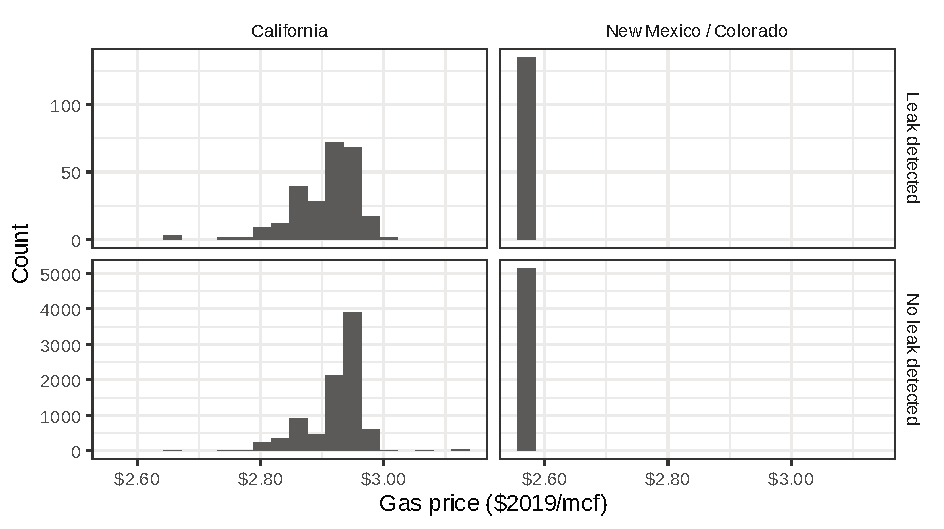
\includegraphics[width=\textwidth]{figureA08_nat_gas_price_histogram.pdf}
\end{figure}



\iftoggle{endfloat}{}{\FloatBarrier} % add a \FloatBarrier if not using endfloat


\newpage

\section{Distribution Fitting}
\label{app:distribution-fitting}

\subsection{Model Priors}
\label{app:model-priors}

We employ a fully Bayesian model, including priors on the parameters we estimate.
As noted in the main text, we choose priors that are very weakly informative on the outcome scale.
Specifically, we chose priors with mean zero and a standard deviation large enough that the predicted value of the outcomes \(e_i\) and \(q_i\) could take any reasonable value.
For \(e_i\), reasonable values are up to perhaps 100~times larger than the largest leak we see.
For \(q_i\), we aimed for a roughly uniform prior distribution by choosing priors of its underlying parameters.
The prior standard deviations are much smaller here;
because of the logit transformation, making the prior standard deviations larger would put a lot of prior weight on probabilities near zero or one
(see \cite{Gelman/etal:2020} for much more discussion).
We use a Student's \(t\) distribution with three degrees of freedom to allow for somewhat more weight in the distributions' tails than the Normal.
Specifically, we de-mean all of the \(X\) variables and use priors of
\(\text{generalized Student's } t(3, 0, 3)\) for each of the leak size parameters \(\beta\) and \(\sigma\).
We use \(\text{Normal}(0, 0.5)\) for the \(A_i\) coefficients \((\psi)\) and
\(\text{Normal}(0, 0.75)\) for the \(\alpha_i\) coefficients \((\phi)\).
While these seem like fairly narrow priors on first glance, these values lead to diffuse priors of the \(A_i\) and \(\alpha_i\).
After the inverse logit transformations described above, the priors on \((\psi)\) and \((\phi)\) are compatible with a wide range of values of  \(A_i\) and \(\alpha_i\).
The prior covariance between coefficients are all zero.

\subsection{Estimated Parameters}
\begin{table}[!bthp] % tab:model-param
\vspace*{-0.5\baselineskip}
\centering
\import{individual_figures/}{tableA03_model_parameters.tex}
\end{table}


\begin{figure}[!bthp]
  \caption{Abatement elasticity \((-\hat{\alpha}_i)\)}
  \label{fig:histogram-alphas}
  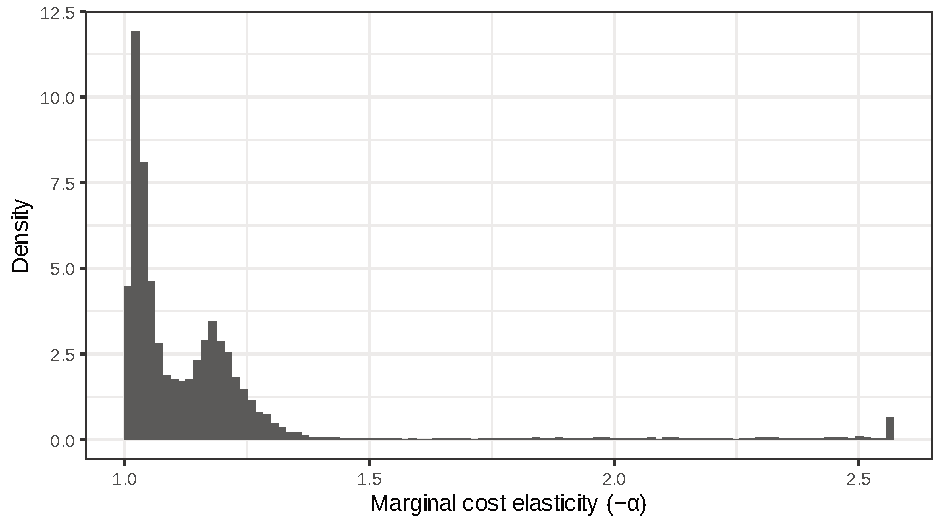
\includegraphics[width=0.99\textwidth]{figureA09_model_cost_alpha_histogram}

The plot shows the mean of \gls{MCMC} draws of each well's \(\alpha_i\), from equation~\ref{eqn:alpha-fitted}.
Values are winsorized at the 99th percentile.
See discussion in section~\ref{sec:fitted-values}.
\end{figure}



\iftoggle{endfloat}{}{\FloatBarrier} % add a \FloatBarrier if not using endfloat



\newpage
\section{Alternative Presentations of Policy Simulation Output}
\label{app:tabular-policy-output}

This section provides tabular versions of figures~\ref{fig:expected-fee-1pct} and \ref{fig:policy-outcomes-1pct}.
Please see those figures and the discussions in sections
\ref{sec:audit-probabilities-and-expected-fees} and
\ref{sec:dwl-and-emissions} for more description.
In these tables, bracketed values indicate 95\% \gls{CI}.

% \ref{tab:expected-fee-1pct}
\import{individual_figures/}{tableA04_expected_fee_1pct_app_table.tex}


% \ref{tab:dwl-emis-1pct}
\import{individual_figures/}{tableA05_policy_outcomes_dwl_emis_app_table_frac=1pct.tex}


\begin{figure}[!bthp]
  \caption{Curvature of \gls{DWL} and Emission Outcomes}
  \label{fig:policy-outcomes-1pct-cardinal}
  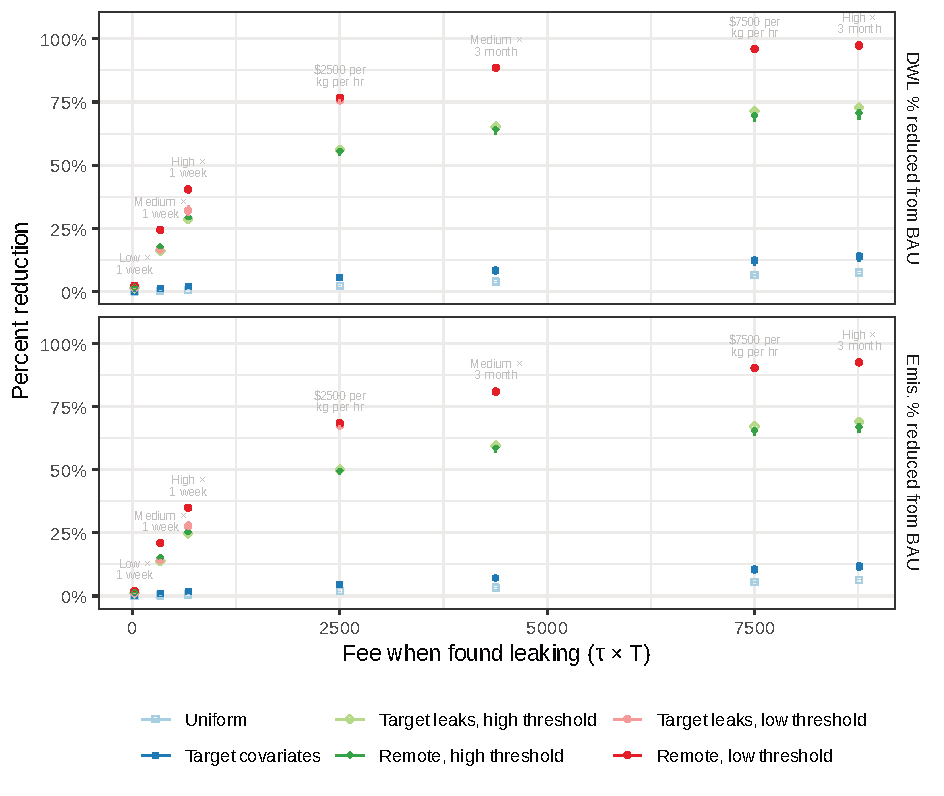
\includegraphics[width=\textwidth]{figureA10_outcomes_dwl_emis_frac=1pct_cardinal}

This graph presents a version of the main-text figure~\ref{fig:policy-outcomes-1pct}, with x-axis values plotted on a cardinal scale, allowing the reader to have a better sense of the curvature of the \gls{DWL} and emissions outcomes at different fee levels.
This plot excludes the case of \(\tau \times T = \text{low} \times \text{3 months}\) for better visualization, as this case is fairly close to \(\tau \times T = \text{med} \times \text{1 week}\).
The plot includes two additional x-axis values, at \(\tau \times T = \) 2500 and 7500, chosen to improve coverage over the x-axis domain.
We present these additional points, rather than a smoother curve, because the computing required for each x-axis value is time-consuming.
\end{figure}

\iftoggle{endfloat}{}{\FloatBarrier} % add a \FloatBarrier if not using endfloat


\newpage
\section{Drilling Response Details}
\label{app:drilling-response-details}

The main text considered the abatement behavior in a fixed population of wells.
However, charging additional fees and increasing abatement costs will make it less profitable to operate a well, and in equilibrium we expect the number of new wells drilled to decline.
This effect ends up being small relative to the per-well abatement.

First, we convert our methane leak fees into their approximate equivalent reduction in well profit from a change in prices.
Briefly, we total the well's expected fee payments and abatement costs, and find the change in commodity price that would result in an equivalent change to well profit, assuming the production quantity is unchanged.
Once we've calculated this price-equivalent change, we borrow supply and demand elasticities from the literature to estimate the change in drilling.
Both the profit-equivalent price change
(\import{tex_fragments/}{intext_OUTCOME=net_private_cost_per_mcf_pct_price_RULE=target_e_high_FRAC=1pct_tauT=high-3month.tex}\%)
and the elasticity of drilling (0.36) are small, so this margin does not substantially affect our conclusions.

This calculation requires stronger assumptions than we applied in the main text.
We consider the extensive margin: wells that face some fee for their emissions will see lower profits, all else equal, than wells that face no fees.
Therefore, fewer wells will be drilled.
It is unlikely that existing wells will stop producing, or that wells will change the amount they produce \parencite{Anderson/Kellogg/Salant:2018}.
To keep things simple, we assume that there's no change in the composition of wells drilled.

To estimate an approximate drilling response, we first translate our expected fees into profit-equivalent changes in the price of natural gas, then we use estimates from the literature of the elasticity of drilling with respect to price.
Further, we assume that a well's cost of drilling does not change in this scenario, except for the cost of abatement.
We also assume that the policy does not lead to any change in the commodity price of natural gas.

To define some notation, say that without any methane policy a well operator spends \(D\) to drill a well, and implement the privately optimal level of abatement.
They earn \(E p_0\) revenue on the well's operation.
Here we elide complications like prices changing over time, uncertainty, and discounting.%
\footnote{%
Here we rely on a martingale price assumption, that today's price is the best guess for tomorrow's price.
Ignoring discounting is less of a problem than it would seem because we consider a change in price that applies to every future period, just as the expected change in profits applies in every future period.
}
With under an audit policy, they still spend \(D\) to drill the well, but now they also spend an additional \(C\) on abatement and \(F\) on expected fees.
Revenue is now \((E + \epsilon) p_0\), since some additional gas may be captured.
We define the profit-equivalent price change as the (lower) price that would result in the same profit the well would earn under the no-policy case.
The profit-equivalent price change is:
\[
\Delta p = \frac{C + F - \epsilon p_0}{E}
\]
For this calculation, we consider considering (\ref{policy-target-e}b), which uses remote measurements to target leaks and a realistic detection threshold.
Using the highest fee we considered (\(\tau = 2\delta\) and \(T\) = 3 months),
we find the production-weighted average price-equivalent is
\import{tex_fragments/}{intext_OUTCOME=net_private_cost_per_mcf_pct_price_RULE=target_e_high_FRAC=1pct_tauT=high-3month.tex}\%
of the wholesale prices in our sample (which are approx. \$2.90--3.90).

For the price elasticity of drilling we rely on \textcite{Gilbert/Roberts:2020}, which calculates that the production-weighted long run elasticity of gas drilling with respect to the Henry Hub gas price is about 0.36 for all onshore drilling in the continental US, or 0.93 for their five-basin focus.
\footnote{%
In table 6 of that paper, the authors report the continental US short-run elasticity of 0.17 (s.e. 0.096), with the coefficient on the lagged dependent variable of 0.53 (s.e. 0.96).
We calculate the approximate long-run elasticity as 0.36 (\hbox{= 0.17 / (1 \(-\) 0.53)}).
}

Combining these, we come to the conclusion presented in the main text.
Even a high-fee policy would see at most a 5--10\% reduction in new (production weighted) drilling, and therefore the changes in expected emissions from this margin are small.

\section{Robustness to Alternative Sets of Variables}
\label{app:robustness-to-alternative-sets-of-variables}

As a robustness check of our specification, we run our analysis for the fee scenario of \(\tau \times T = \delta \times \text{3 months}\) using all subsets of our preferred set with at least two variables (56~specifications), plus combinations that use sub-basin fixed effects and inverse hyperbolic sine number of wells within 10~km (3~specifications \footnote{(1) our main
specification with basin dummies replaced by sub-basin cluster dummies, (2) our main
specification plus the number of wells within 10 km, and (3) both.}).


The sub-basin fixed effects are modeled by \gls{DBSCAN}, an unsupervised learning technique that assigns well pads to clusters and outliers.
\gls{DBSCAN} works by identifying clusters as regions of high density that are separated by regions of low density.
In contrast to counting the number of wells within a fixed radius, \gls{DBSCAN} can handle irregular geographic distributions of wells.
We used geospatial coordinates to cluster, and selected \gls{DBSCAN} parameters to provide subjectively reasonable-looking cluster patterns.
We end up with four clusters in the densely drilled San Joaquin basin, six in the rest of California, and one large cluster in the San Juan basin.
When we use these fixed effects in the regressions, we include one fixed effect level per cluster, and one level for each basin's outliers.
By including the sub-basin fixed effects and/or the number of wells within 10 km, our aim is to control for the well density information that was not accounted for in our preferred specification.

In figure~\ref{fig:robustness-reg-spec}, the preferred specification is in black and the other specifications are in gray.
The points for the preferred specification are qualitatively similar to the others. There are a few features to note here.
The range across specifications is quite narrow: roughly 10 percentage points from the lowest to the highest.
The confidence intervals here overlap substantially.
From these features, we conclude that our takeaways do not depend dramatically on the particular specification choice, at least among the variables included.



\begin{figure}[!bthp]
  \caption{Comparison across specifications}
  \label{fig:robustness-reg-spec}
  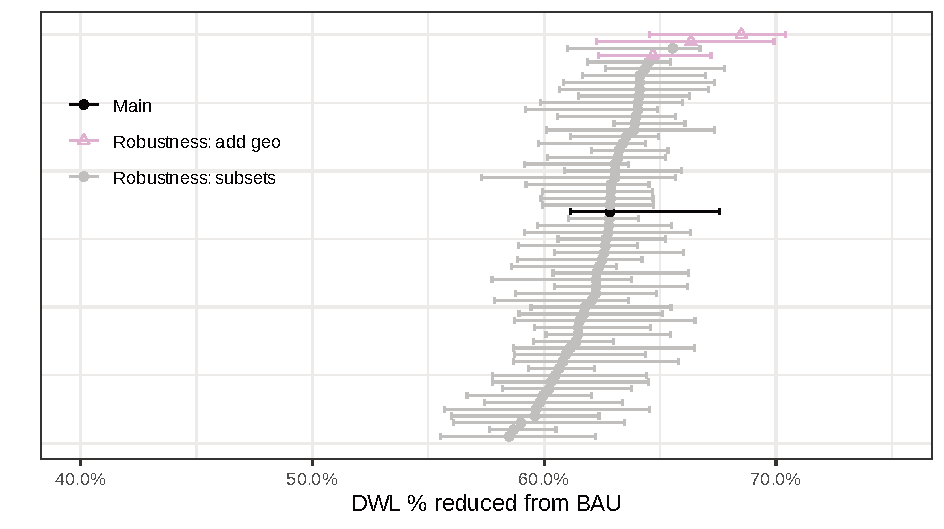
\includegraphics[width=\textwidth]{figureA11_robustness_audit_result_dwl_rule=target_e_high_frac=1pct_tauT=med-3month}
  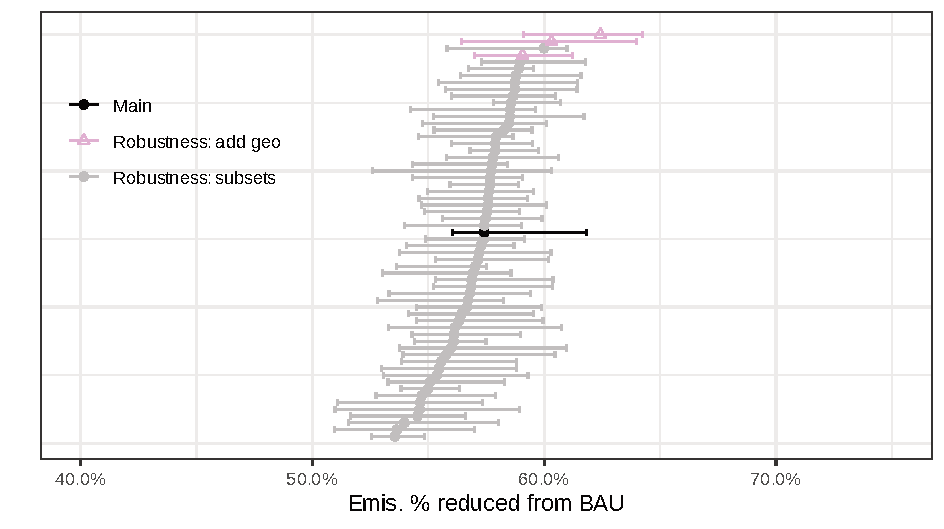
\includegraphics[width=\textwidth]{figureA11_robustness_audit_result_emission_rule=target_e_high_frac=1pct_tauT=med-3month}

The top and bottom panels plot the change in \gls{DWL} and emissions for the case of \(\tau \times T = \delta \times \text{3 months}\).
The black point is our preferred specification
(see variables in table~\ref{tab:model-param}).
The gray and pink points are alternative specifications, using subsets of the main specification and additional geographic variables.
These specifications are described in in appendix section~\ref{app:robustness-to-alternative-sets-of-variables}.
Bars indicate 95\% \gls{CI}.
To save computation resources, both the estimates and the confidence intervals are derived from standard \gls{MCMC} values, as opposed to the more computationally intensive BayesBag procedure employed in the main results of the paper.
These non-bootstrapped CIs are qualitatively similar to, and are slightly larger than, the bootstrapped CIs reported in figure~\ref{fig:policy-outcomes-1pct}.
\end{figure}


\newpage

\begin{RaggedRight}
\singlespacing
\twocolumn


\printbibliography[notkeyword={code}, heading=subbibliography]

\newpage

\nocite{base}
\nocite{arrow}
\nocite{cmdstanr}
\nocite{curl}
\nocite{data.table}
\nocite{dplyr}
\nocite{fs}
\nocite{furrr}
\nocite{future}
\nocite{ggplot2}
\nocite{ggpattern}
\nocite{glue}
\nocite{gt}
\nocite{here}
\nocite{igraph}
\nocite{jsonlite}
\nocite{lubridate}
\nocite{magrittr}
\nocite{matrixStats}
\nocite{nngeo}
\nocite{posterior}
\nocite{powerjoin}
\nocite{processx}
\nocite{purrr}
\nocite{RColorBrewer}
\nocite{readxl}
\nocite{remotes}
\nocite{rlang}
\nocite{sf}
\nocite{stringr}
\nocite{tibble}
\nocite{tidyr}
\nocite{tidyselect}
\nocite{units}
\nocite{unix}
\nocite{xml2}
\nocite{python-numpy}
\nocite{python-pandas}
\nocite{python-python3}
\nocite{python-black}
\nocite{python-snakemake}
\nocite{python-cmdstan}
\nocite{python-Ipopt}
\nocite{python-scikit-learn}
\nocite{python-SciPy-NMeth}


\printbibliography[keyword={code}, heading=subbibliography, title={Software Citations}]
\end{RaggedRight}
\end{document}
